%%
% このファイルは筑波大学情報学群情報科学類の卒業研究論文のサンプルです。
% このファイルを書き換えて、このサンプルと同様の書式の論文をLaTeXを使って
% 作成できます。
%
% OSやLaTeXの設定によっては漢字コードや改行コードを変更する必要があります。
%%
\documentclass[a4paper,11pt]{jreport}

%%【PDF, PostScript, JPEG, PNG等の画像の貼り込み】
%% dvipdfmx を使う場合
\usepackage[dvipdfmx]{graphicx}
%% dvipdfmx を使ってPDFの「しおり」を付ける場合
%%\usepackage[dvipdfmx,bookmarks=true,bookmarksnumbered=true,bookmarkstype=toc]{hyperref} \usepackage{pxjahyper}
\usepackage{ulem}
\usepackage{times} % use Times font instead of default one
\usepackage{algorithm}
\usepackage{algpseudocode}

\setcounter{tocdepth}{3}
\setcounter{page}{-1}

\setlength{\oddsidemargin}{0.1in}
\setlength{\evensidemargin}{0.1in}
\setlength{\topmargin}{0in}
\setlength{\textwidth}{6in}
%\setlength{\textheight}{10.1in}
\setlength{\parskip}{0em}
\setlength{\topsep}{0em}

\newcommand{\figref}[1]{図\ref{#1}}
\newcommand{\tabref}[1]{表\ref{#1}}
\newcommand{\secref}[1]{\ref{#1}節}
\newcommand{\algorithmref}[1]{Algorithm \ref{#1}}

%% タイトル生成用パッケージ(重要)
\usepackage{coins}

%% タイトル
\title{TODO: タイトル}
%% 著者
\author{岡部 純弥}
%% 指導教員
\advisor{岡 瑞起, 阿部 洋丈}

%% 年度と主専攻名
\fiscalyear{2023}
\majorfield{ソフトウェアサイエンス主専攻}

\begin{document}
\maketitle
\thispagestyle{empty}
\newpage

\thispagestyle{empty}
\vspace*{20pt plus 1fil}
\parindent=1zw
\noindent
%%
%% 論文の要旨
%%
\begin{center}
{\Large \bf 要  旨}
\vspace{2cm}
\end{center}

優れた輻輳制御アルゴリズムを発見することは難しい。主な理由として、コンピュータネットワークの構造が時々刻々と変化することが挙げられる。つまり、特定のネットワーク構造化で最適なアルゴリズムを探索しても、時間経過につれ、良いパフォーマンスを発揮できなくなってしまう。

そこで、大規模言語モデルと進化アルゴリズムを用いることで任意のネットワーク環境下で最適化を行う探索手法を提案する。既存の探索手法では、探索空間の制約が厳しかったものの、大規模言語モデルを用いることで、この問題を解決できた。

TODO: 事実確認

実際にネットワークシミュレータを用いた実験を行い、ベンチマークを超える輻輳制御アルゴリズムを発見できた。

%%%%%
\par
\vspace{0pt plus 1fil}
\newpage

\pagenumbering{roman} % I, II, III, IV
\tableofcontents
\listoffigures
%\listoftables

\pagebreak \setcounter{page}{1}
\pagenumbering{arabic} % 1,2,3

\chapter{序論}

\section{研究背景}

TCP/IPネットワークでは、トランスポート層で輻輳制御が行われている。輻輳制御の難しさとして、限られた観測可能な値から、観測不可能な状態を推定しなければならないことが挙げられる。
つまり、限られた観測値から、輻輳が発生しているのかを判断したうえで、パケット送信量を制御しなければなければならない。

さらに、ネットワーク構造が変化し続けているため、支配的なアルゴリズムが存在することもなく、数年に一度はパラダイムシフトが起こっている。

現在の輻輳制御アルゴリズムの探索、発見は、ヒューリスティックに行われている側面があり、人的リソースを割き続けなければらない。つまり、ネットワーク構造の変化に柔軟に対応可能な探索手法の発見が求められている。

\newpage

\section{本論文の構成}

第2章の前半では、輻輳制御アルゴリズムの概要や、その発展について述べる。
第2章の後半では、近年の大規模言語モデルの発展や、その応用について概説する。特に、輻輳制御アルゴリズムの探索手法として、大規模言語モデルを用いることの可能性について述べる。
第3章では、これらの関連研究を踏まえたうえでの仮説、および提案手法について述べる。
第4章では、仮説を検証するために提案手法の実装、実験の詳細について述べる。
第5章では、実験結果を示し、その結果に対する考察を行う。
第6章では、本論文のまとめと今後の課題について述べる。

\newpage

\chapter{関連研究}
\section{輻輳制御アルゴリズム}

\subsection{輻輳制御アルゴリズムの概要}

% TODO: 表現の見直し
パケット交換型の通信網である、TCP/IPネットワークでは、トランスポート層で輻輳制御が行われている。
そもそも輻輳とは、コンピュータネットワークのあるノード
\footnote{多くの場合、これは中継ルータのいずれかである。}
上で、パケットが過剰に蓄積されることを指す。
一般的に、ルータ上ではパケットを蓄積するためのバッファが存在しており、これは FIFO: First In First Out 型のキューであるため、このバッファが溢れるとパケットのロスが発生する。
TCP/IPにおいて、トランスポート層では通信の信頼性を確保するために、パケットロスを検知すると、パケットが再送される。
このため輻輳が発生すると、パケットロスが発生し、通信のスループットが低下する。
\footnote{よりひどい状態になると、輻輳崩壊と呼ばれる状態になり、大規模な通信障害を引き起こすこともある。}
このような状態を回避するために、輻輳制御という仕組みが存在する。

輻輳制御\cite{congestion-avoidance}は、観測可能な値からネットワークの状態を推定し、パケット送信量を制御することで、輻輳を回避する。
\footnote{実際にJacobson\cite{congestion-avoidance}で提案された、世界初の輻輳制御アルゴリズムは、TCP Tahoeと名付けられた。}
また、万が一輻輳が発生した場合には、輻輳制御アルゴリズムは輻輳が発生していることを検知しパケット送信量を制御する。
興味深いことに、Kellyら\cite{kelly1998rate}は、全体最適化やゲーム理論の観点から、各々のノードが自身のパケット送信量を制御することで、全体としてのスループットを最大化できることを示した。
それゆえ、現在の輻輳制御アルゴリズムは、多くの場合、OSのカーネルに実装されており、自分自身のパケット送信量を制御のみを行う。

極めて単純な輻輳制御アルゴリズムの動作を\algorithmref{algorithm:congestion_control_algorithm}に示す。
\begin{algorithm}
  \caption{Basic Congestion Control Algorithm}
  \label{algorithm:congestion_control_algorithm}
  \begin{algorithmic}[1]
  \State $windowSize \gets 1$
  \State $threshold \gets veryLargeNumber$
  \While{true}
      \If{ACK is received}
        \If{$windowSize < threshold$}
            \State $windowSize \gets windowSize + 1$
        \Else
            \State $windowSize \gets windowSize \times 2$
        \EndIf
      \EndIf
      \If{Congestion is detected}
          \State $threshold \gets windowSize / 2$
          \State $windowSize \gets 1$
      \EndIf
  \EndWhile
  \end{algorithmic}
\end{algorithm}
\algorithmref{algorithm:congestion_control_algorithm}では、以下の2つの変数と、ACKの受信によってパケットの送信量を制御する。
\begin{description}
  \item[windowSize]
  \item[] windowSizeは、一度に送信可能なパケットの数を表す。輻輳制御アルゴリズムは、このwindowSizeを制御することで、パケット送信量を制御する。
  \item[threshold]
  \item[] thresholdは、windowSizeを指数関数的に増加させる際の閾値を表す。thresholdを超えた場合には、windowSizeは加算によって増加させる。
\end{description}
つまり、\algorithmref{algorithm:congestion_control_algorithm}では、輻輳が発生していない場合には、windowSizeを指数的あるいは線形に増加させることで、パケット送信量を増加させる。
一方で、輻輳が発生した場合には、windowSizeを減少させることで、パケット送信量を減少させる。
これが、輻輳制御アルゴリズムの基本的な動作である。

\subsection{代表的な輻輳制御アルゴリズム}

ここでは、代表的な輻輳制御アルゴリズムについて概説する。
輻輳制御アルゴリズムは、大きくLoss-basedとDelay-basedに分類される。
これは輻輳制御アルゴリズムが、どのように輻輳を検知するかによって分類されており、Loss-basedはパケットロスを検知することで輻輳を検知する。
一方で、Delay-basedは、パケットの遅延を検知することで輻輳を検知する。
それぞれの代表的な輻輳制御アルゴリズムについて、\figref{figure:congestion_control_classification}に示す。

\begin{figure}[htbp]
  \centering
  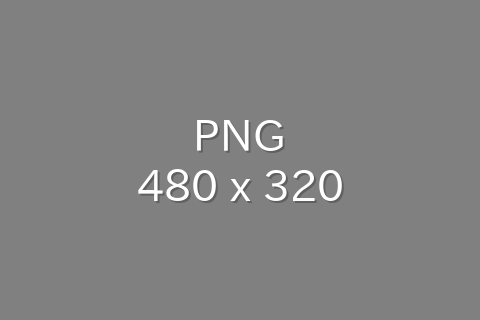
\includegraphics[width=0.6\linewidth]{fig/chap02/empty.png}
  \caption{輻輳制御アルゴリズムの分類}
  \label{figure:congestion_control_classification}
\end{figure}

Loss-basedの代表的な輻輳制御アルゴリズムとしては、TCP Reno\cite{reno,tcp}が挙げられる。
これは、TCP Tahoe\cite{congestion-avoidance}を改良したもので、fast retransmitとfast recoveryという機構を追加したものである。
\footnote{TODO: 補足する}

\begin{figure}[htbp]
  \centering
  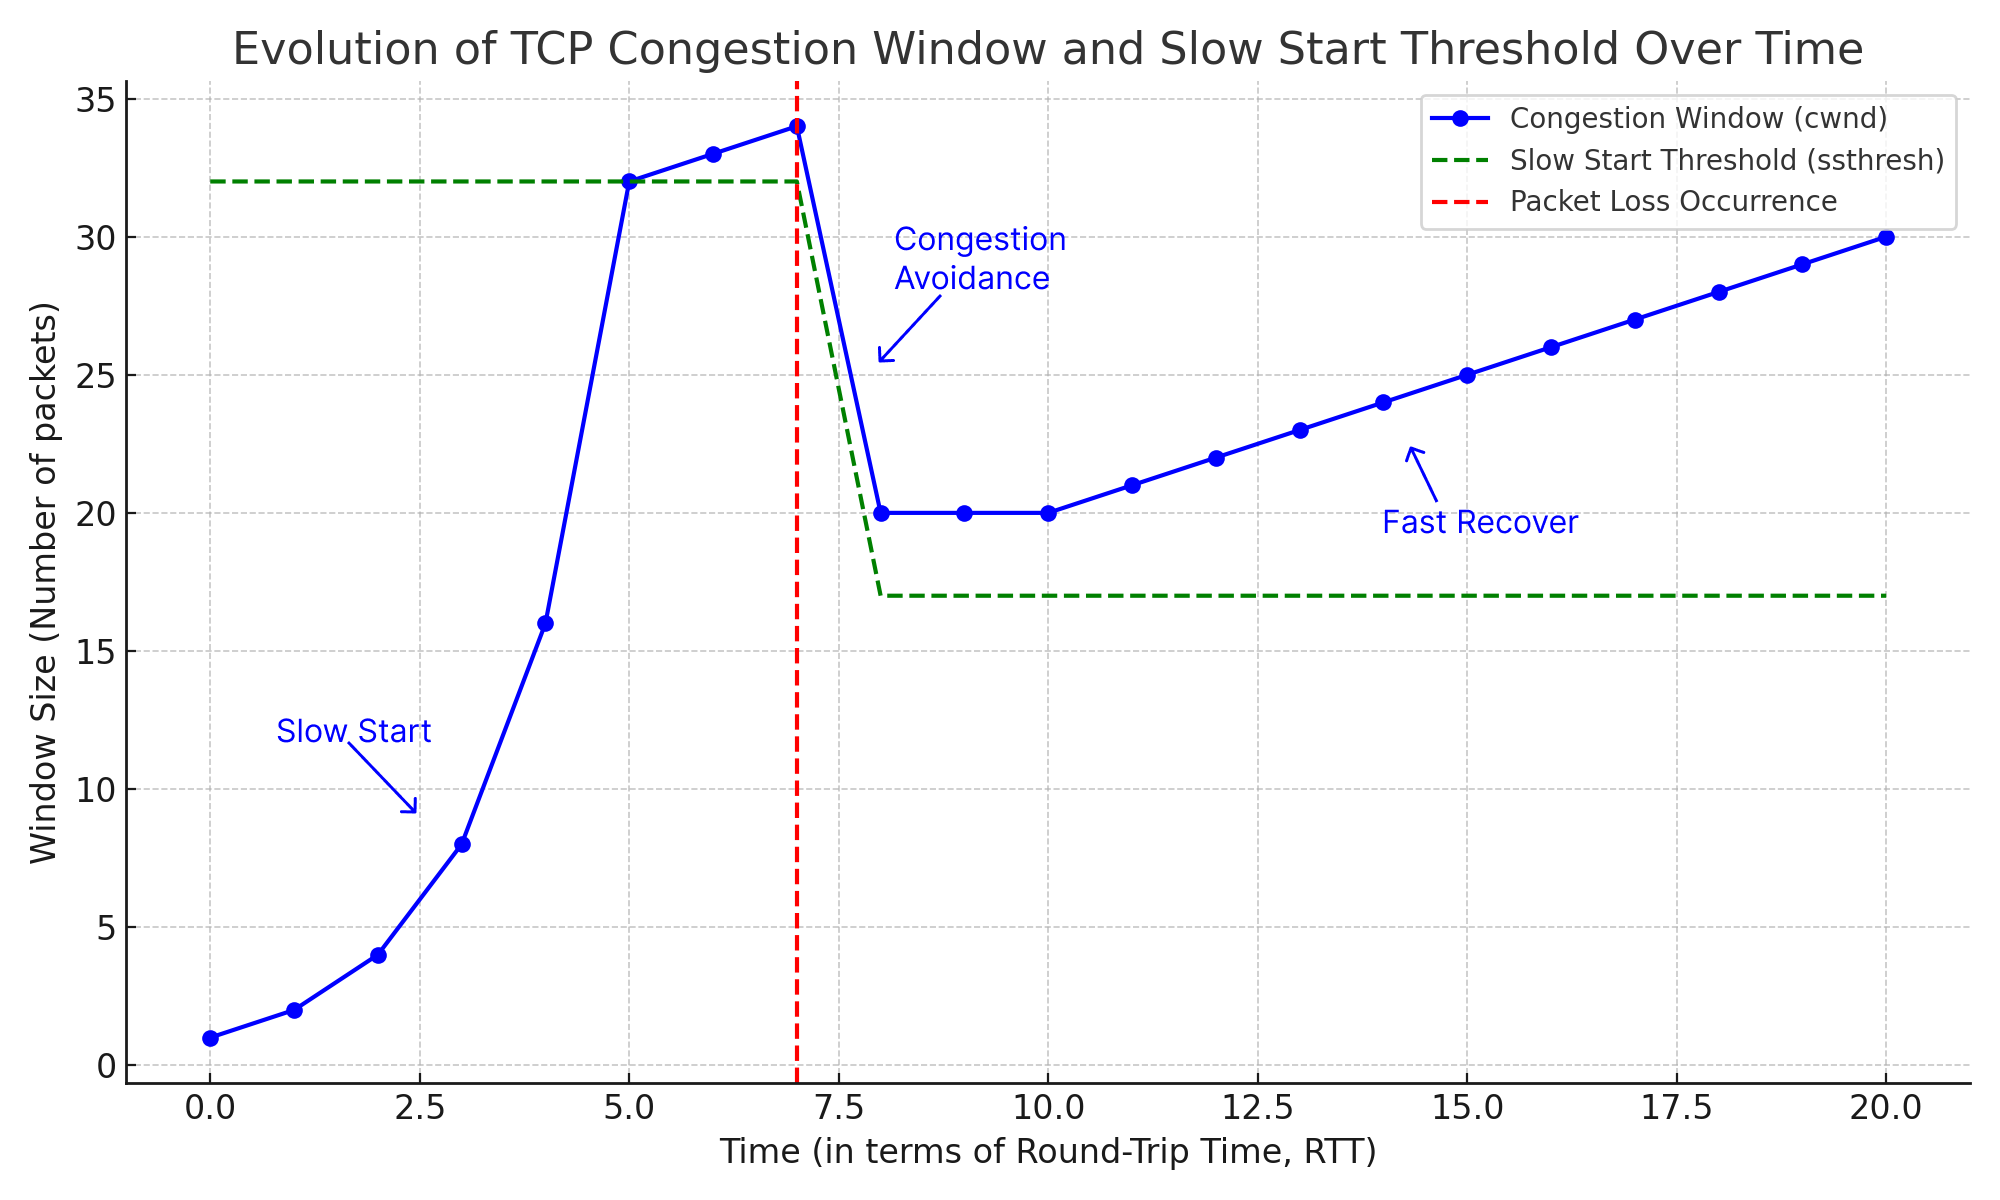
\includegraphics[width=0.6\linewidth]{fig/chap02/CongestionControlAlgorithm_Timeline.png}
  \caption{TCP Renoの動作の概要}
  \label{figure:reno-timeline}
\end{figure}

一方で、Delay-basedの代表的な輻輳制御アルゴリズムとしては、TCP Vegas\cite{tcp-vegas}やBBR\cite{bbr}が挙げられる。

より詳細な輻輳制御アルゴリズムの概説については、Lowら\cite{980245}, Ghaffari\cite{GHAFFARI2015101}などを参照されたい。

\section{大規模言語モデルと進化アルゴリズム}

\subsection{大規模言語モデル}

Attention: Vaswaniら\cite{attention}

BERT: Devlinら\cite{devlin2019bert}

GPT3: Brownら\cite{gpt3}

\subsection{進化アルゴリズム}

GA: Whitleyら\cite{genetic-algorithm} Voseら\cite{vose1999simple}

GA survey: Katochら\cite{katoch2021review}

\subsection{進化アルゴリズムへの大規模言語モデルの応用}

LMX: Meyersonら\cite{meyerson2023language}

ELM: Lehmanら\cite{lehman2022evolution}

\subsection{進化アルゴリズムの輻輳制御アルゴリズムへの応用}

Endoさんの論文: \cite{endo-2022-toward}

\newpage

\chapter{形式}

ここでは、論文の表紙および本体の記述方法について述べる。

\section{表紙}

表紙は、以下の各項目に相当する文字列を記述した上で、\texttt{$\backslash$maketitle}により作成する。

\begin{description} \parskip=1pt
\item{題目: }
題目は\texttt{$\backslash$title}に記述する。行替えを行う場合には $\backslash \backslash$ を入力する。
ただし、題目の最後に$\backslash \backslash$ を入力するとコンパイルが通らなくなるので注意する。
なお、題目が複数行に渡るなどの理由により表紙ページがあふれた場合にはスタイルファイルを変更する必要がある。
\item{著者名: }
著者名は\texttt{$\backslash$author}に記述する。
\item{指導教員名: }
指導教員名は\texttt{$\backslash$advisor}に記述する。
2名以上の場合には複数名を記述する。
\item{主専攻名: }
主専攻名は\texttt{$\backslash$majorfield}に記述する。「○○主専攻」という形式にすること。
\item{年度: }
年度は\texttt{$\backslash$fiscalyear} に記述する。年度は提出時のものを記述すること。
\end{description}

\section{本体}

本体は1段組で記述する。

図表には番号と説明(caption)を付け、文章中で参照する。
表~\ref{table:scores}と図~\ref{figure:smile}はそれぞれ
表と図の例である。表の説明は表の上に、図の説明は図の下に書くことが多い。
図の挿入に用いる \LaTeX のパッケージについては使用環境に合わせて自由に選択してほしい。

\begin{table}[hbt]
\caption{表の例}
\label{table:scores}
\begin{center}
\begin{tabular}{|c|r|r|r|r|}
\hline
年度 & 1年次 & 2年次 & 3年次 & 4年次 \\
\hline
2016 & 85 & 92 & 86 &  88 \\
2017 & 83 & 89 & 90 & 102 \\
2018 & 88 & 87 & 91 & 112 \\
\hline
\end{tabular}
\end{center}
\end{table}
\medskip

レポートや論文の書き方、日本語の\LaTeX の使い方に関しては、Web 上の情報や
参考書など~\cite{Bibunsho,ScienceResearchWriting}を参照のこと。
また、参考文献、図、表の入れ方を含む、文章のスタイルについては、
ACM, IEEE, 情報処理学会, 電子情報通信学会などの学会が出版している
ジャーナルや国際会議の論文のスタイルを参考にするとよい。

\chapter*{謝辞}
\addcontentsline{toc}{chapter}{\numberline{}謝辞}

本研究を行うにあたって、研究テーマの決定、研究内容の議論、外部発表の機会の提供など、様々な形でご指導を頂いた岡瑞起准教授、阿部洋丈准教授の両先生に深く感謝を申し上げます。
また、同研究プロジェクトの中で議論した、岡研究室の矢内千陽さん、OSSS研究室の佐藤創太さんの両氏にも感謝を申し上げます。
ネットワークシミュレータの取り扱いや実験環境に関して、OSSS研OBの森越さんには多大なるご協力を頂きました。
実験用のマシンのセットアップ等に関して、OSSS研の山本さん、広瀬さんには大変お世話になりました。
この場を借りて、深く御礼申し上げます。

そして、日々の研究活動やミーティングにおいて、様々な形でご協力を頂いた岡研究室の皆様、OSSS研究室の皆様にもあらためて感謝申し上げます。

\newpage

\addcontentsline{toc}{chapter}{\numberline{}参考文献}
\renewcommand{\bibname}{参考文献}

%% 参考文献に jbibtex を使う場合
\bibliographystyle{junsrt}
\bibliography{ref.bib}
%% [compile] jbibtex sample; platex sample; platex sample;

%% 参考文献を直接ファイルに含めて書く場合
\begin{thebibliography}{1}
\bibitem{Bibunsho}
奥村 晴彦, 黒木 裕介.
\newblock LaTeX2ε美文書作成入門 改訂第7版.
\newblock 技術評論社, 2017.

\bibitem{ScienceResearchWriting}
Hilary Glasman-Deal.
\newblock Science Research Writing: A Guide for Non-Native Speakers of English.
\newblock Imperial College Press, 2009.
\end{thebibliography}

\end{document}
